\clearpage
\section{New fitting: physical channels 1--4}
The owner fitted four CFD simulators on1--4, kept the RJ45 order and connected
both USB pairs on4: DAC0/1 to J8 ADC, DAC2/3 to J6 integrator. Shared monitor
outputs remain on the SMU. Finite discovery confirms slot7 ports0/1/2/3 to PM4/3/2/1.
Initially PM IPbus was unavailable and MCU reported FPGA not ready. Fresh DNA
and MCU1803 were verified; qualified ff2f746c was restored to volatile SRAM.
No build, MCU/CPLD/flash or PLL programming. Kasli HDMI outputs stay driven.
\subsection{Recorded coverage}
\begin{center}\begin{tabular}{rllllll}\toprule
Channel & ADC/bits & Integrator & TDC & Phase & Monitor & B/C/D\\\midrule
1 & NM/NM & NM & PASS & PASS & PASS & PASS\\
2 & NM/NM & NM & PASS & PASS & PASS & PASS\\
3 & NM/NM & NM & PASS & PASS & PASS & PASS\\
4 & PASS/PASS & INC & PASS & PASS & PASS & PASS\\
\bottomrule\end{tabular}\end{center}
NM means not measured; INC means incomplete. USB remains4; analog1--3 awaits
cable moves. Integrator6 retains its INCOMPLETE result. Previous selected IDs
and sealed raw evidence are unchanged. PASS covers functional assembly checks.
\subsection{Channel4 analog response}
The first channel4 route guard did not show the expected DAC0/1 response and
stopped before the full ADC/integrator sequence. The owner then reported a reboot;
observed PGOOD loss interrupted monitor collection, and PM FPGA became not ready.
Qualified SRAM was restored again. Interrupted data remain excluded; fresh monitor
and internal-DAC acquisitions use new directories. TDC and phase completed before
the reboot and retain that epoch. Channel4 status is given explicitly in the table.
Full ADC method, when qualified, uses257points per bank over plus/minus1.2V
at1V common mode; integrator method uses13coarse/26fine points and independent
returns/plus-minus5mV controls. An independent J6 test may proceed while J8 route
verification is incomplete. No response or ambiguous traces do not establish a defect.
\begin{center}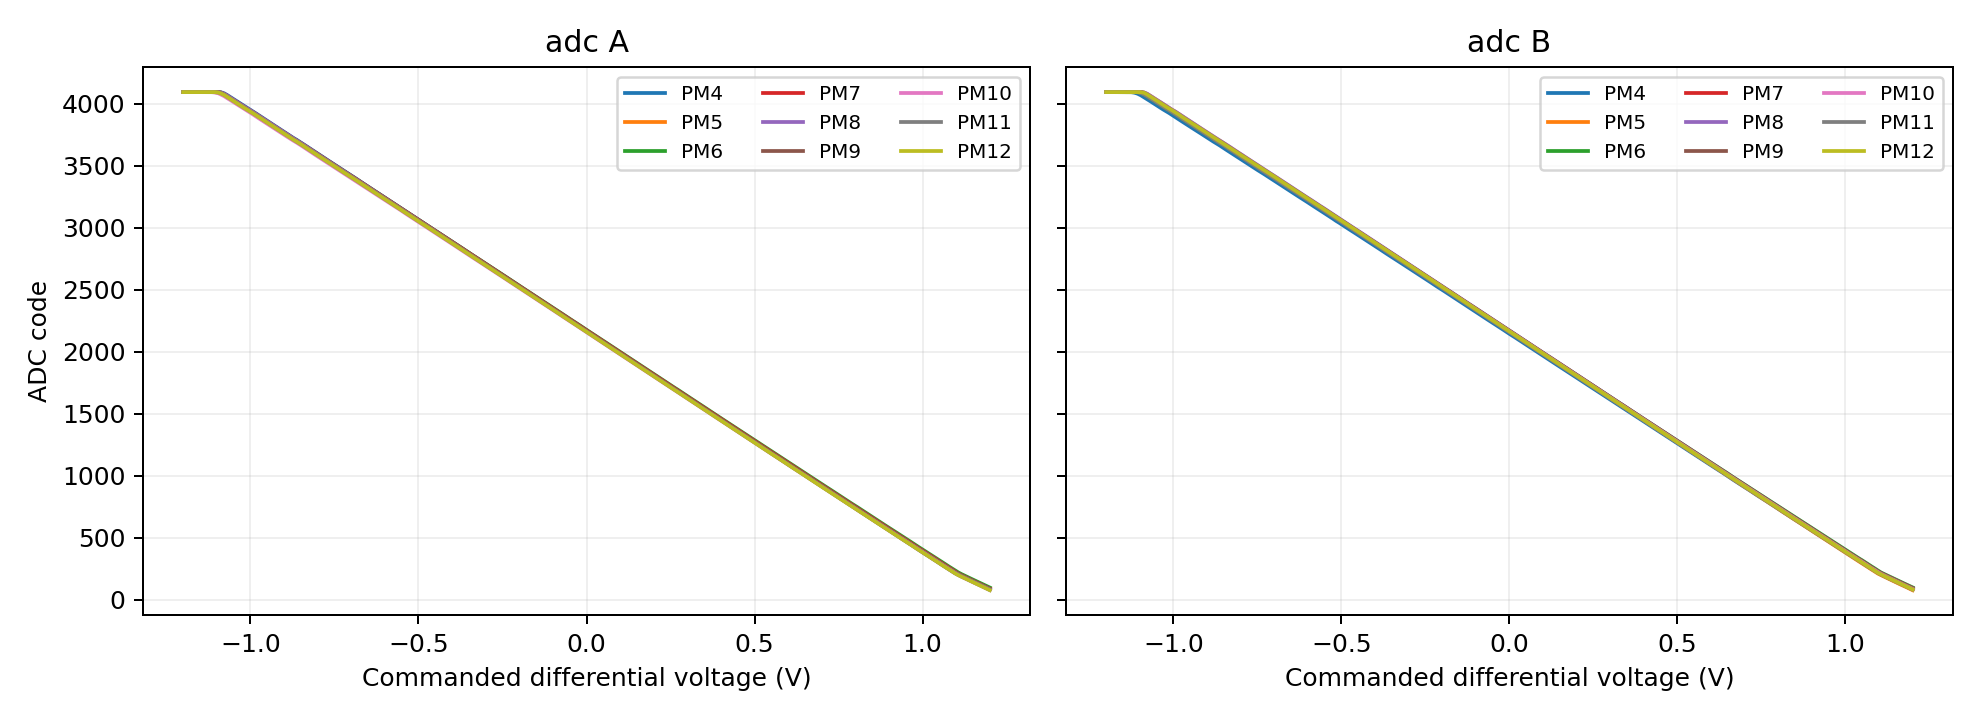
\includegraphics[width=\linewidth]{group14-adc-common.png}\end{center}
\begin{center}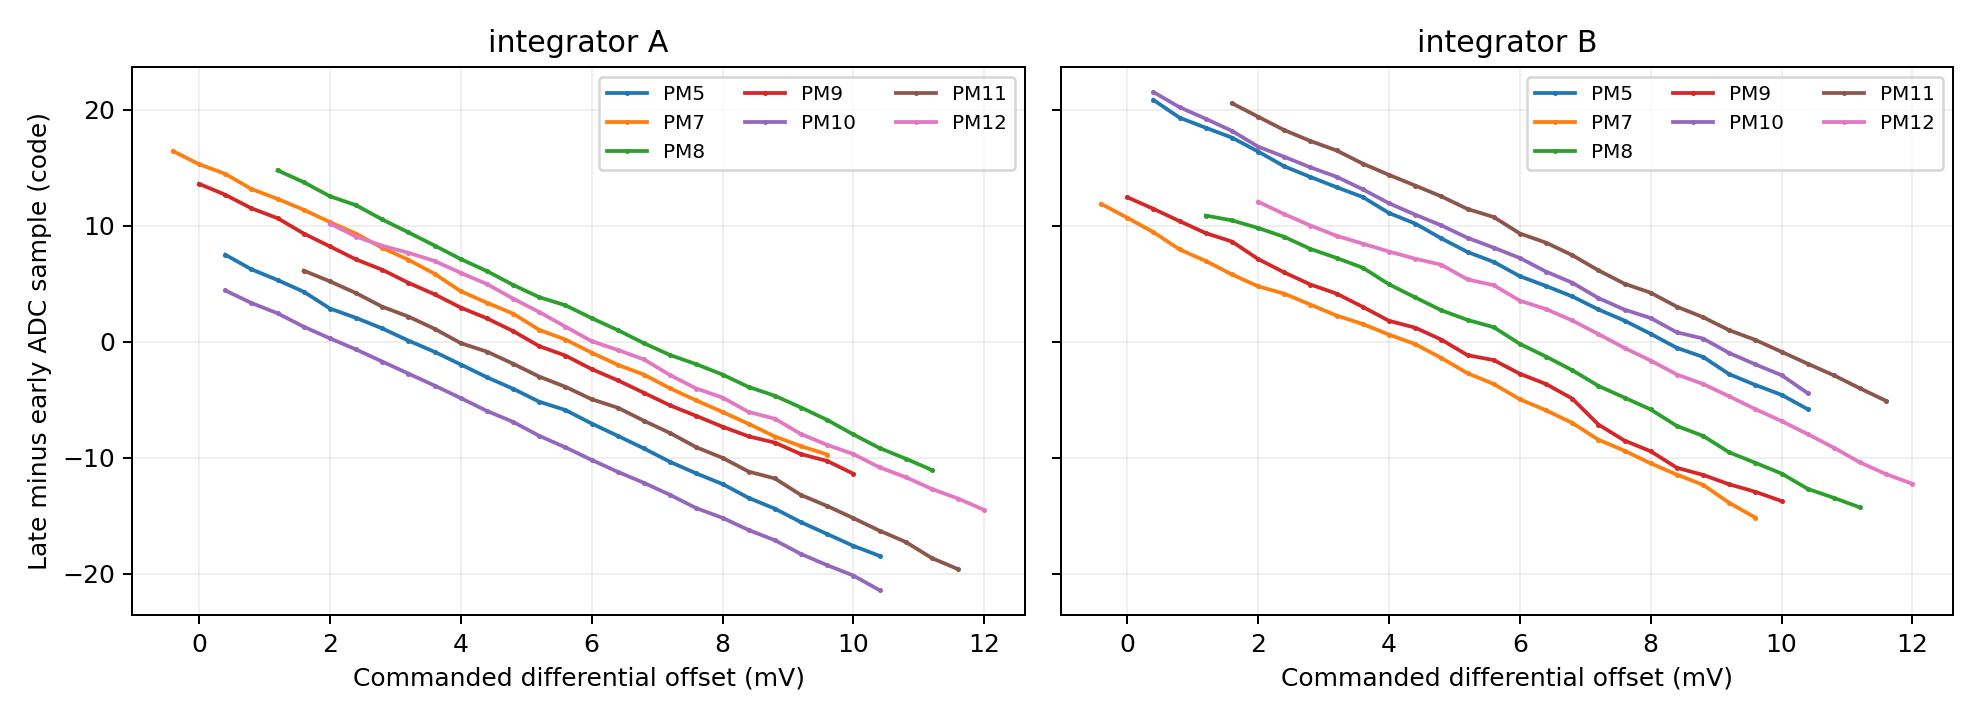
\includegraphics[width=\linewidth]{group14-integrator-common.png}\end{center}
Only qualified labelled channels are overlaid. Integrator6 remains excluded.
Older10--12 use c7c42d28, newer analog uses ff2f746c; receipts retain epochs.
Commanded voltages are whole-chain observations, not calibrated ADC-only gain.
\subsection{All12 channels: TDC and gate phase}
Clock40 tests include finite discovery, quiet windows, count1/64/512/1024 and
25phase positions per port. Raw13-bit words and count conservation are checked.
Historical9--12 TDC uses the corrected-clock14November capture; withdrawn c7
clock qualification is excluded. Gate phase uses101DAC-A codes per module,
both return lanes and nominal24sampler bins per LHC period. Discontinuities
remain visible; no absolute calibration or intrinsic jitter claim.
\begin{center}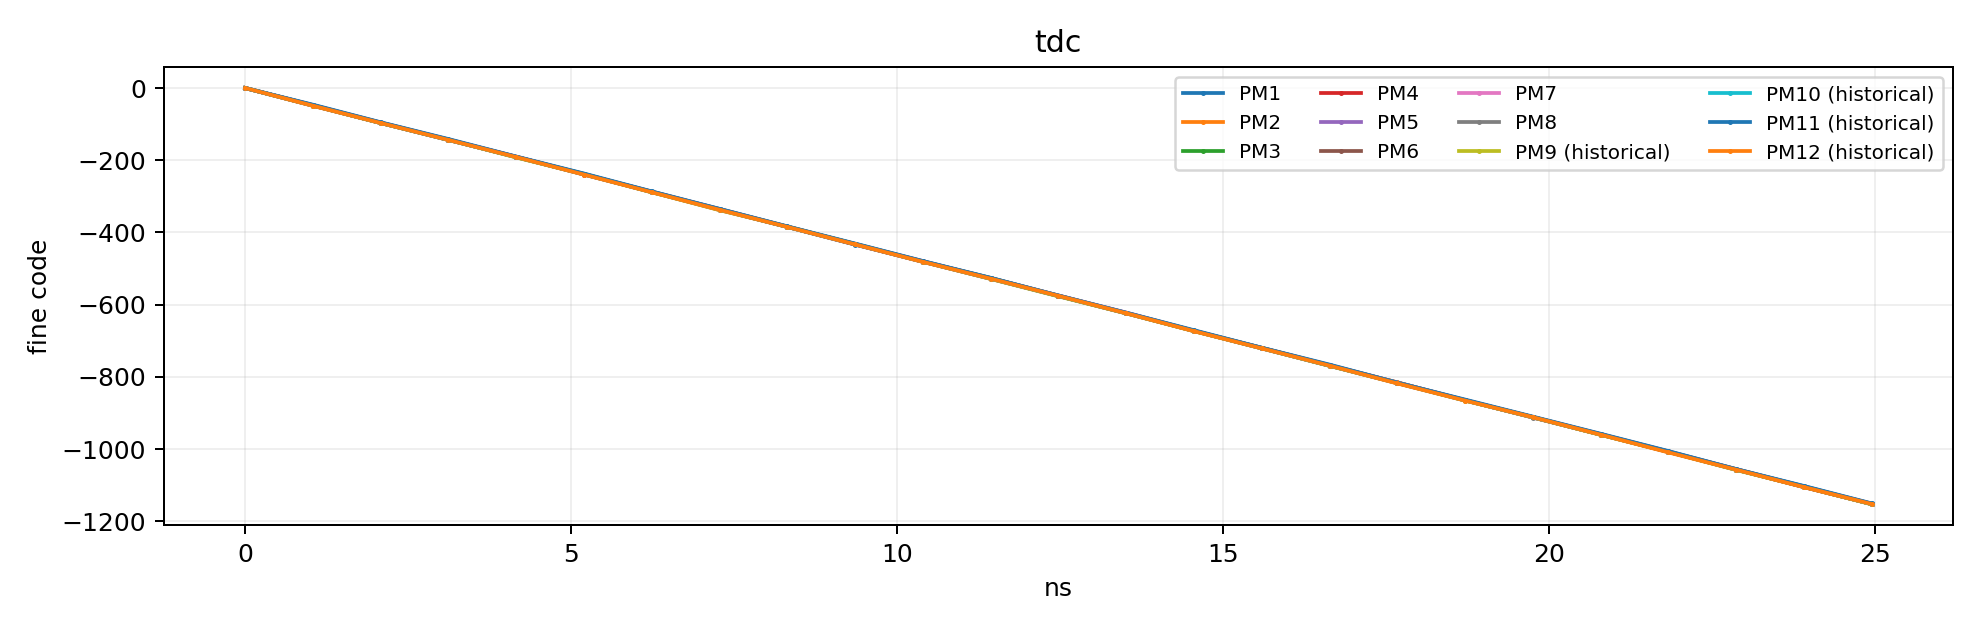
\includegraphics[width=\linewidth]{group14-tdc-01-12.png}\end{center}
\begin{center}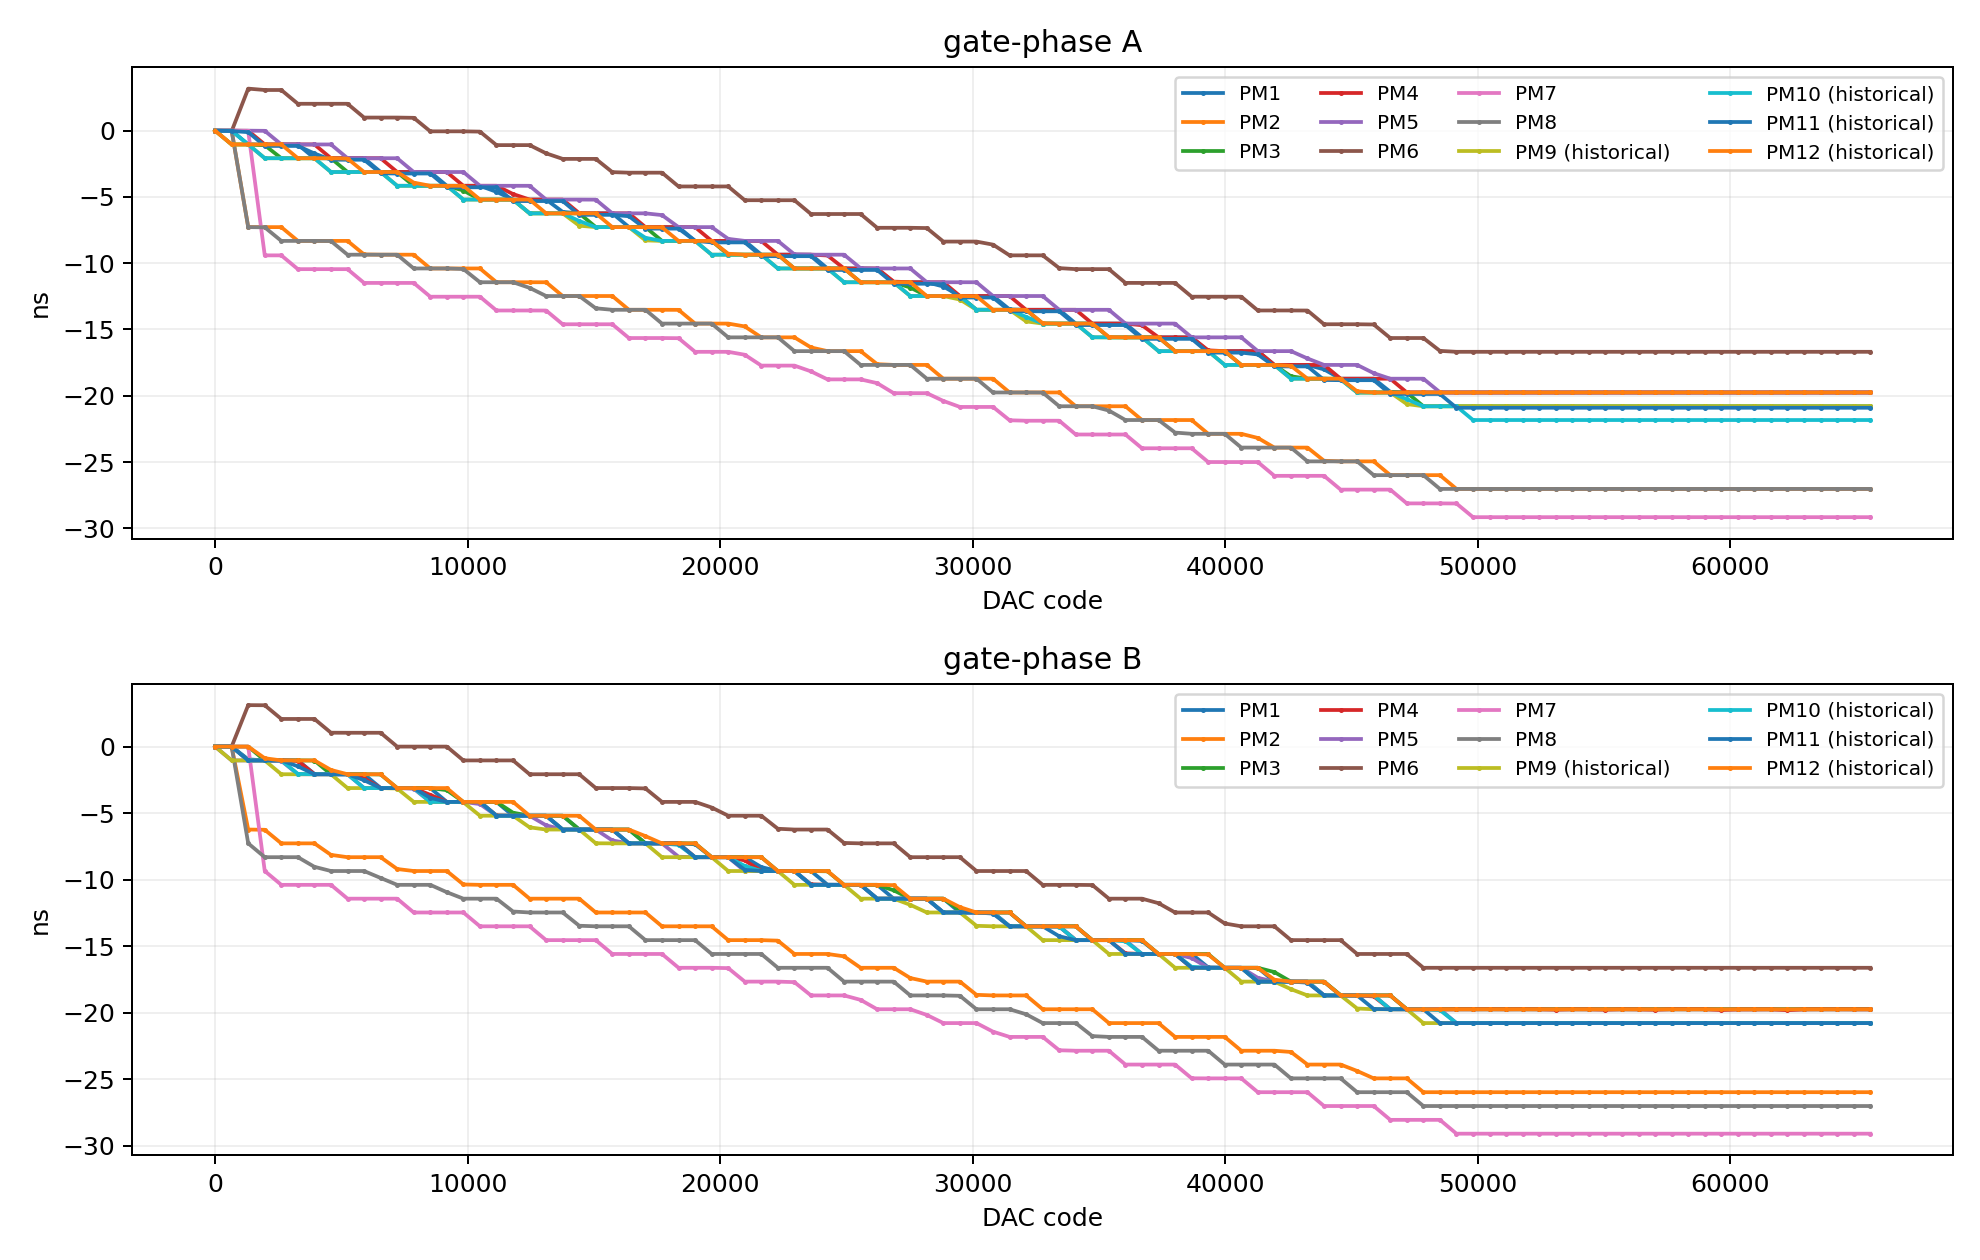
\includegraphics[width=\linewidth]{group14-gate-phase-01-12.png}\end{center}
\subsection{Shared SMU monitors and internal DACs}
Eight monitor inputs per module, three fresh readings each, were recorded with
SMU0A/local Force HI/LO. Negative/positive supply dividers use nominal53/33.
Only one shared monitor mux is active at a time. Internal B/C/D scans each use
101codes and3fresh readings; all12-channel transfer curves below retain epochs.
\begin{center}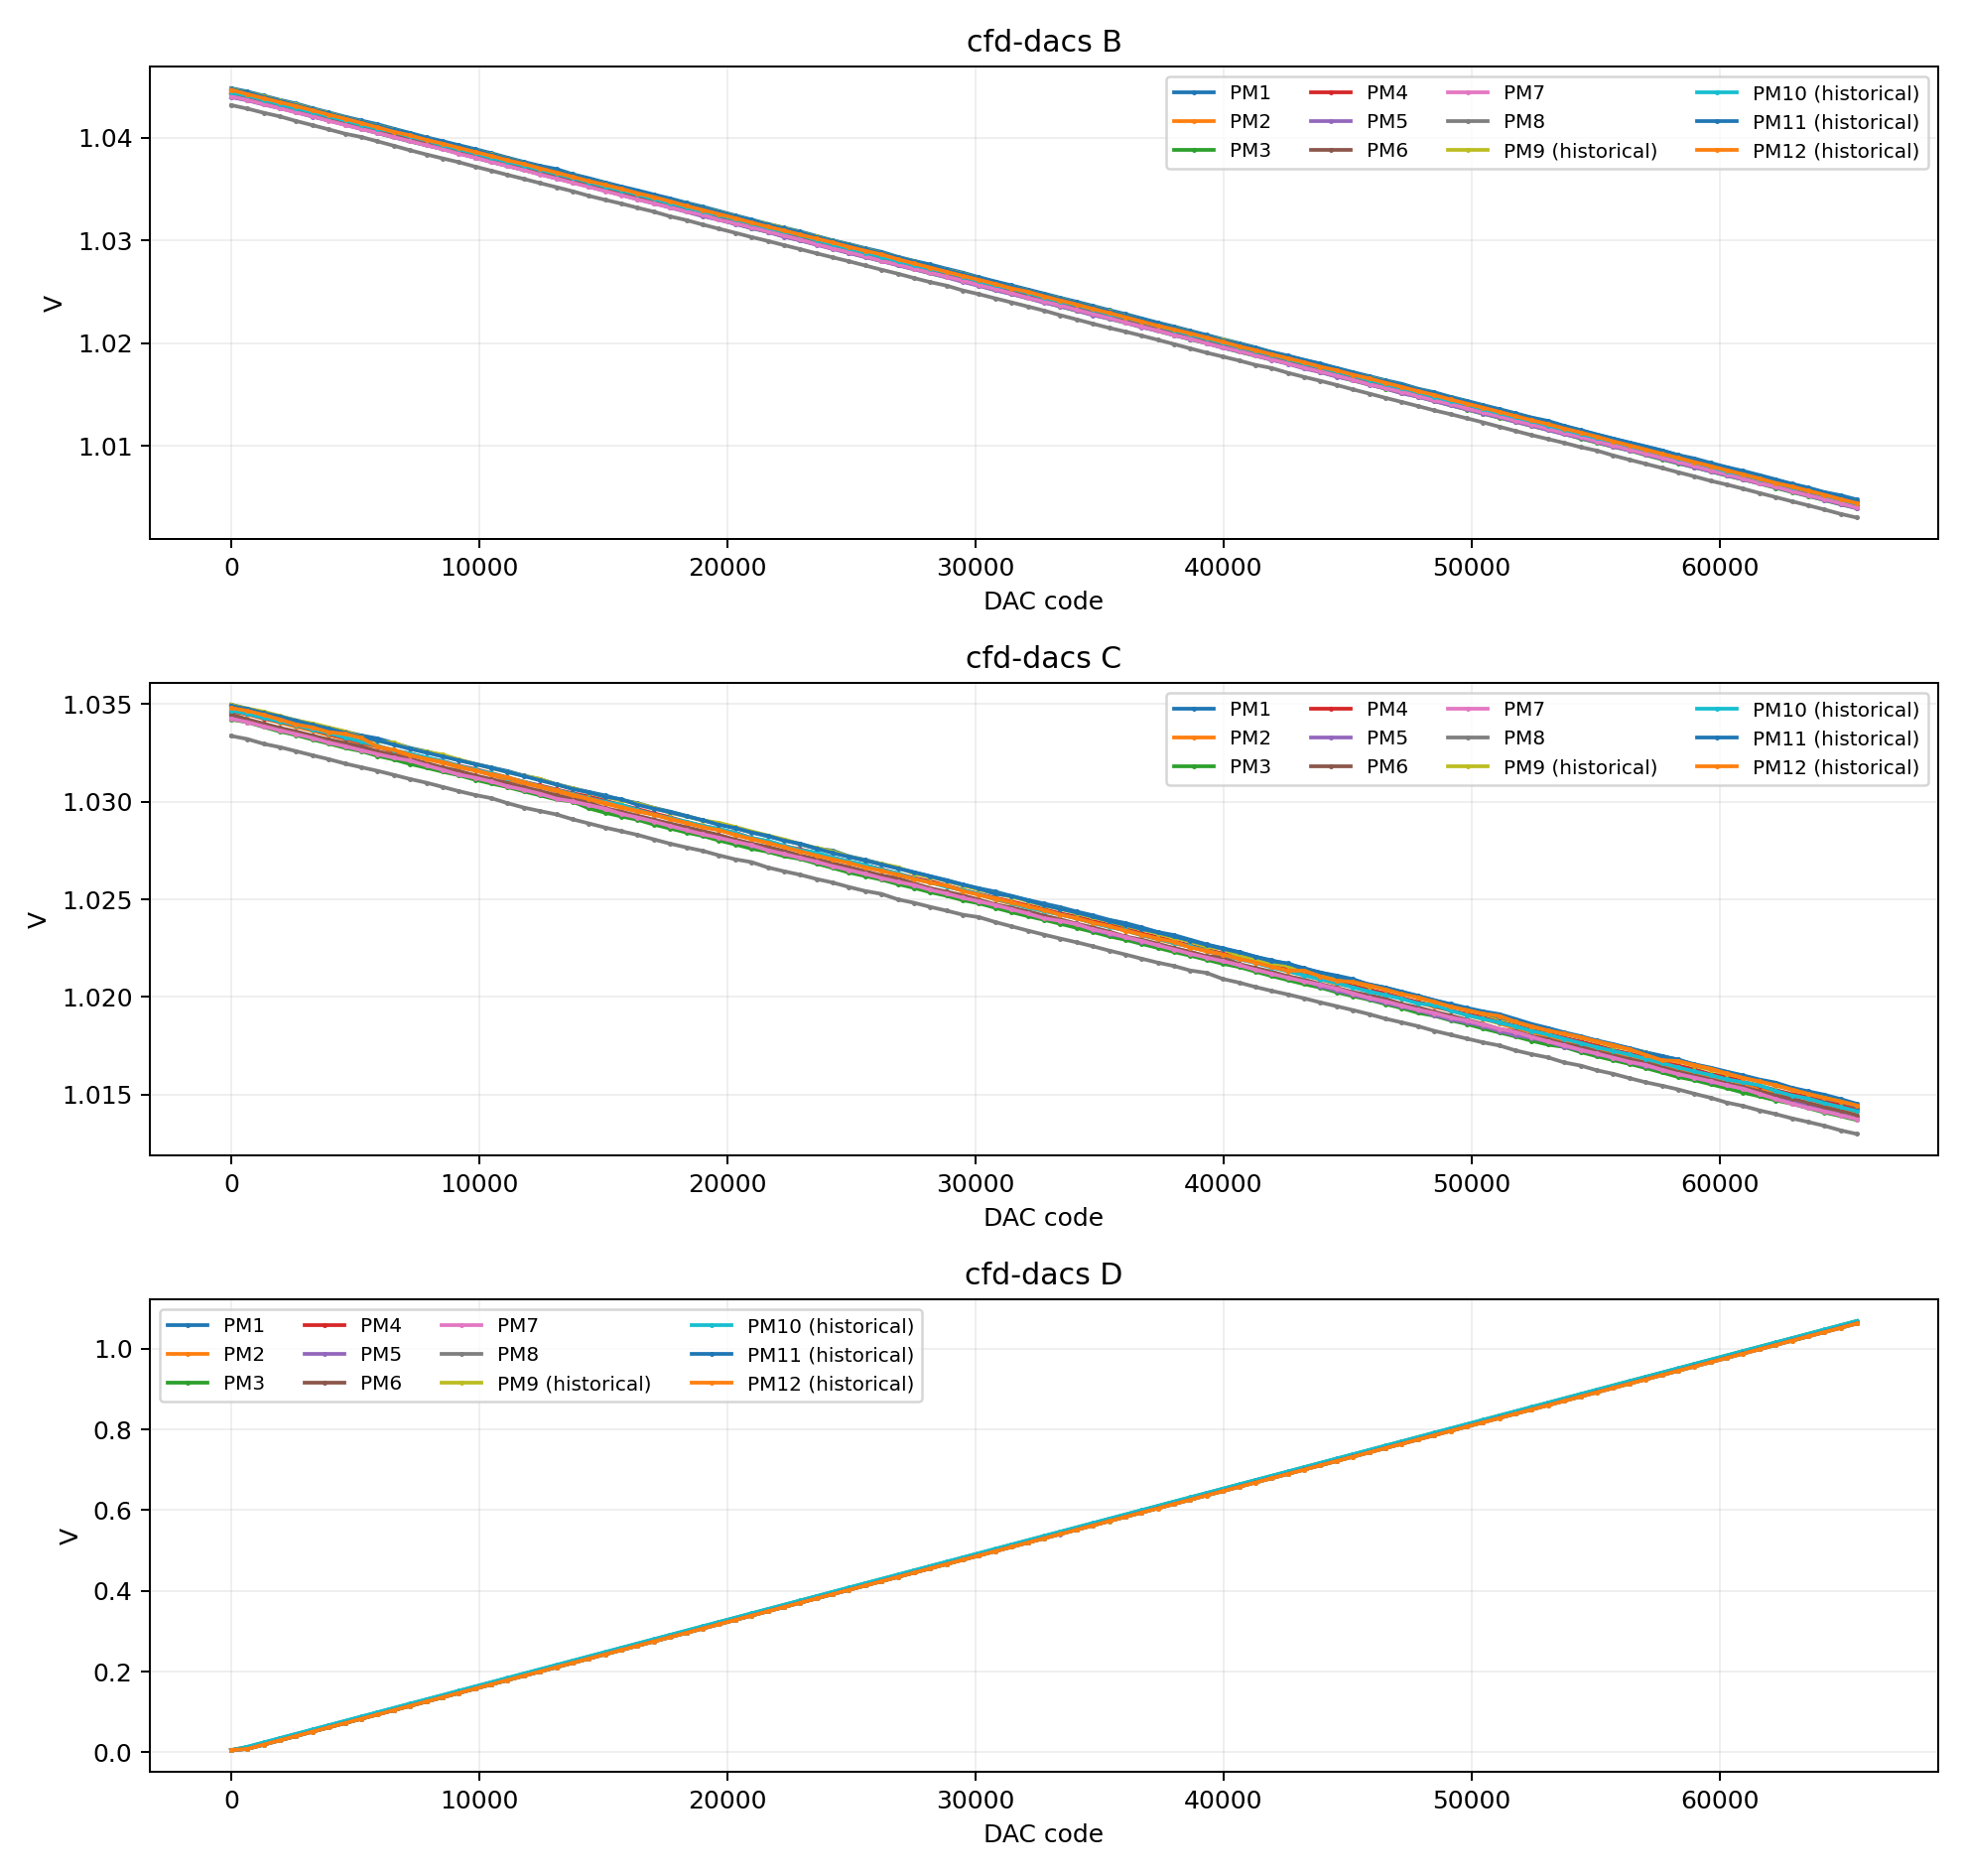
\includegraphics[width=\linewidth]{group14-cfd-dacs-01-12.png}\end{center}
Final SMU OFF/HIZ, auto-on OFF. All four monitor muxes inhibited/TCA0;
exercised internal DACs restored0000. External park/GPIO recorded in raw files.
Kasli outputs retained, leases released. Source contracts and raw inventory verified.
\subsection{Zero-input waveforms and FFT, qualified channels shown}
Separate local capture origins, not synchronized traces. FFT one-sided RMS code
per bin at nominal80.1574MS/s, not PSD or intrinsic aperture-jitter measurement.
\begin{center}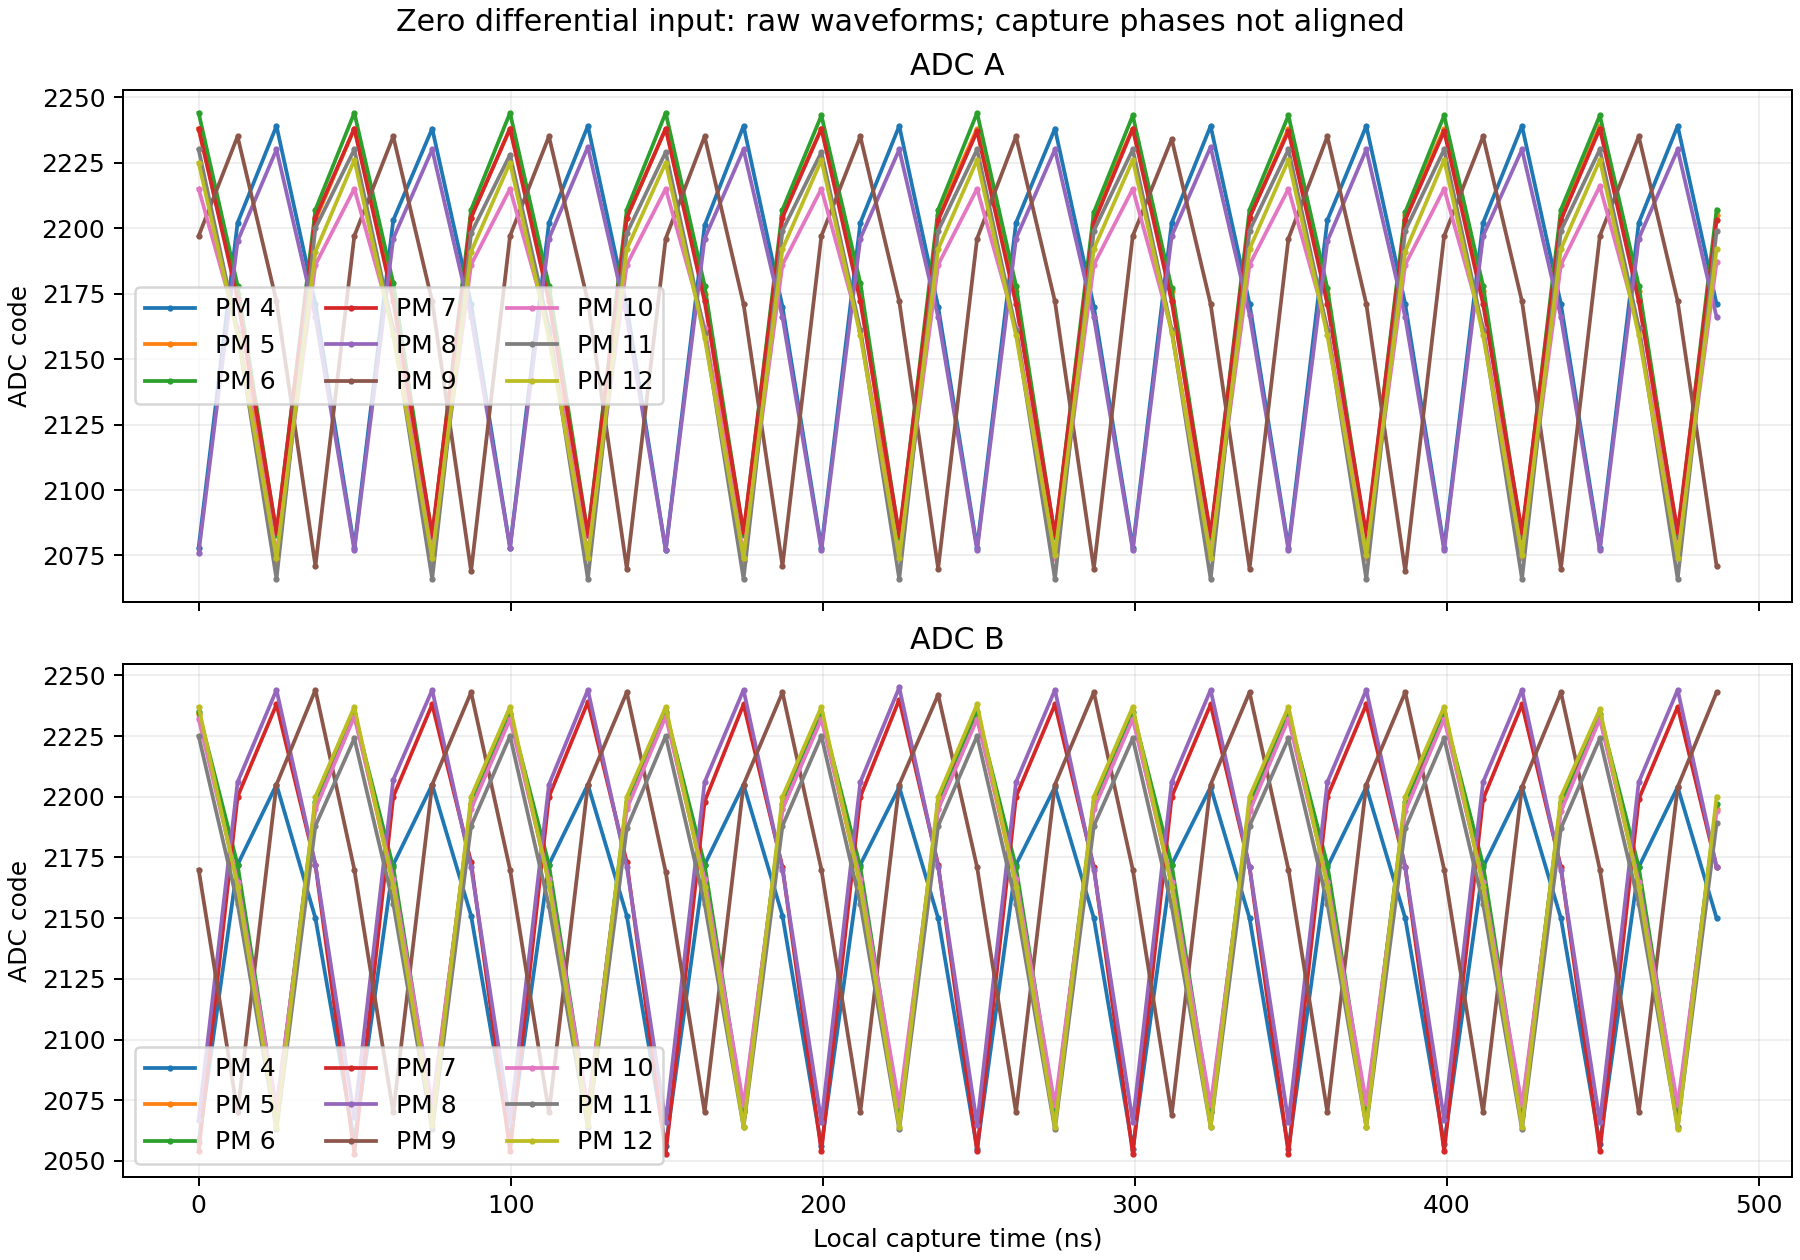
\includegraphics[width=\linewidth]{group14-adc-zero-time.png}\end{center}
\begin{center}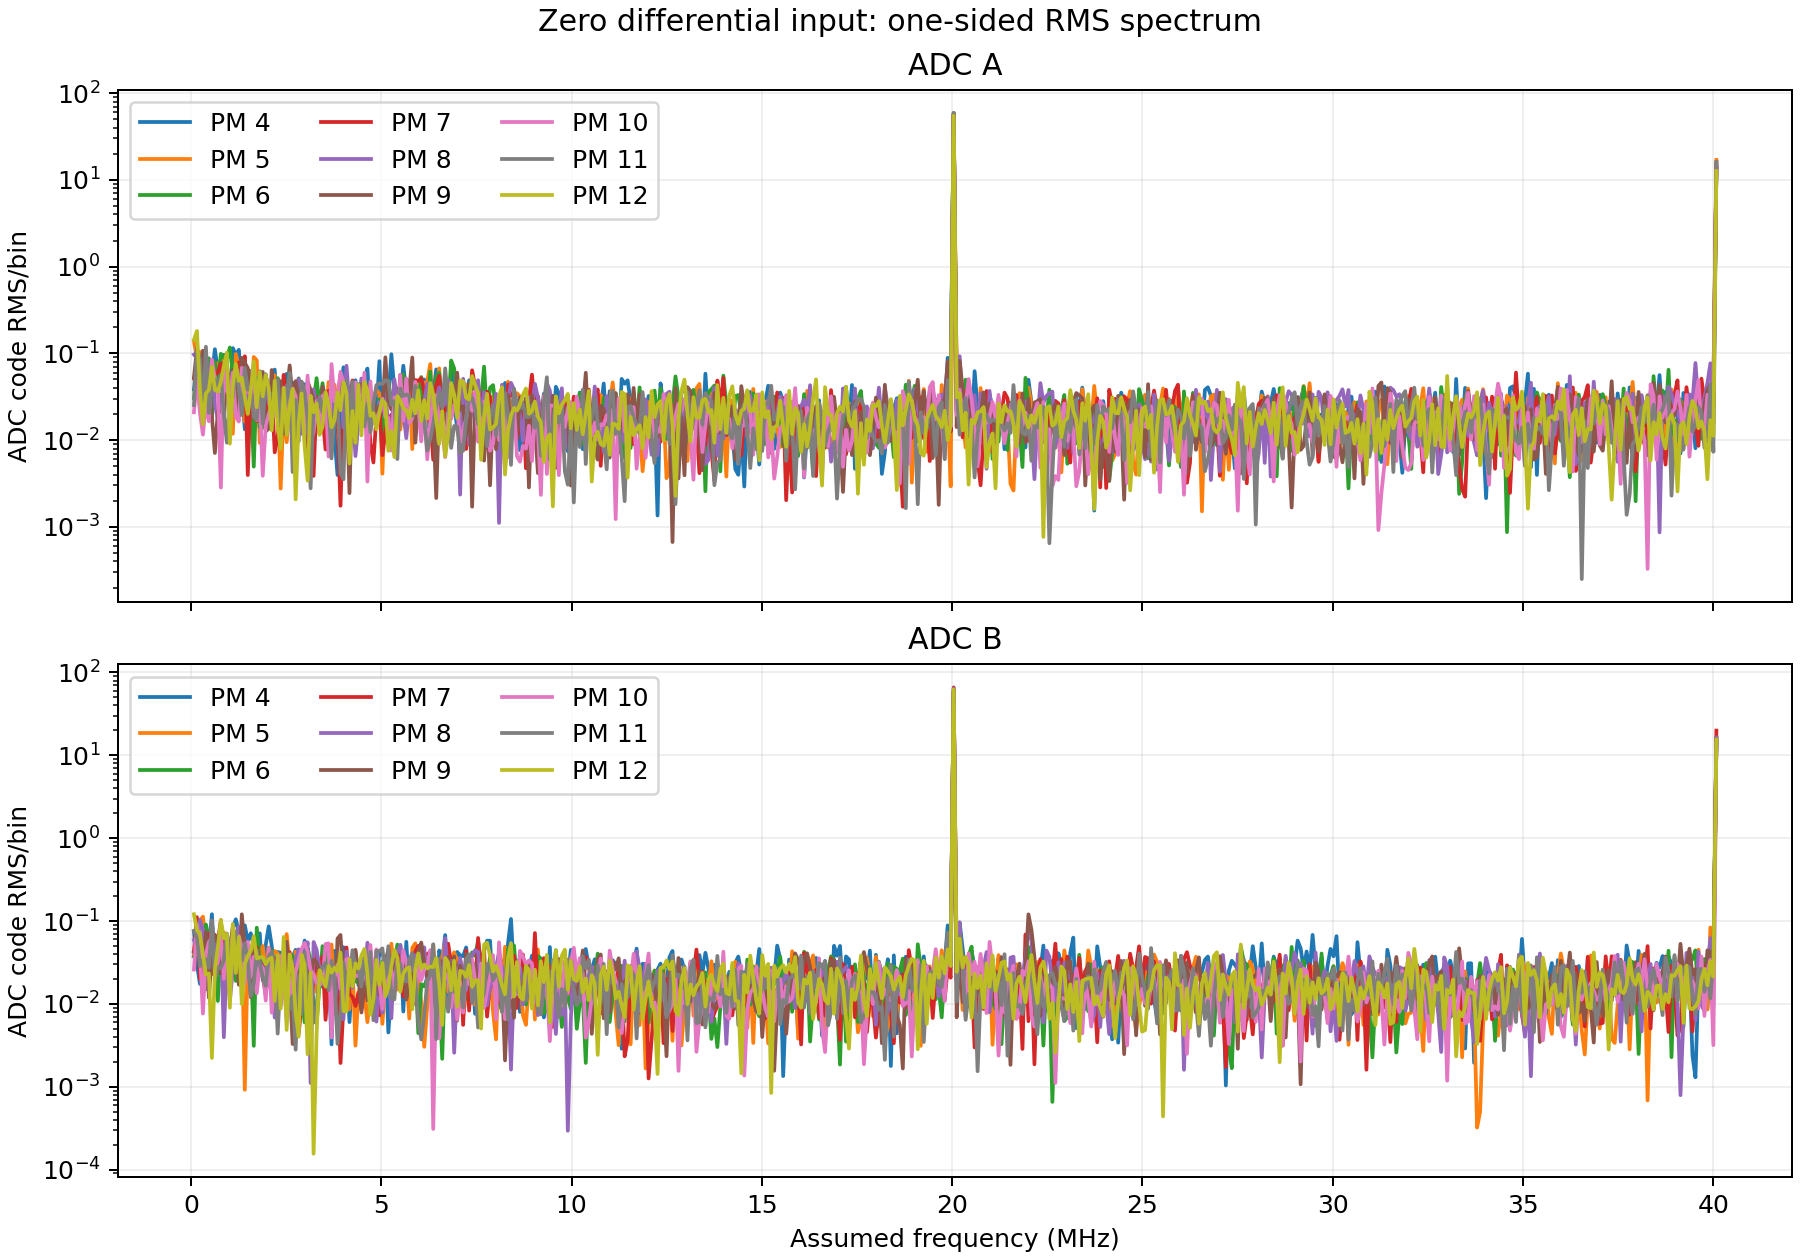
\includegraphics[width=\linewidth]{group14-adc-zero-fft.png}\end{center}
\subsection{Numerical results for the new fitting}
\begin{center}\begin{tabular}{lrrrr}\toprule
Monitor(V) & PM1 & PM2 & PM3 & PM4\\\midrule
CFD\_OFFSET & +1.03503 & +1.03456 & +1.03419 & +1.03461\\
CFD\_CMP\_OFFSET & +0.00533 & +0.00515 & +0.00541 & +0.00522\\
BUFFER\_OFFSET & +1.02480 & +1.02439 & +1.02396 & +1.02434\\
DRV\_OFFSET & +1.04479 & +1.04438 & +1.04398 & +1.04431\\
DRV\_VOCM & +1.53691 & +1.53638 & +1.53569 & +1.53636\\
N5V5\_PM12 & -5.51089 & -5.50990 & -5.51056 & -5.50336\\
P1V3 & +1.30052 & +1.31292 & +1.29981 & +1.30091\\
P5V5\_PM12 & +5.47961 & +5.47397 & +5.47067 & +5.46785\\
\bottomrule\end{tabular}\end{center}
Values are corrected to monitored nodes, including nominal supply divider53/33;
three fresh SMU readings per input, not traceable calibration.
\begin{center}\begin{tabular}{lrrr}\toprule
ADC4 & Gain(code/V) & Zero mean(code) & Template-removed RMS(code)\\\midrule
A & -1788.60 & 2172.085 & 0.687 \\
B & -1766.34 & 2145.790 & 0.691 \\
\bottomrule\end{tabular}\end{center}
After the reboot, independent active/inhibited probes verified the declared J8
route. Only the complete post-reboot acquisition is selected; the first no-response
probe remains diagnostic history. No ADC defect is inferred from that first probe.
\subsection{Integrator4 incomplete: raw waveforms}
The two coarse attempts both lacked a unique bank-B signed crossing. Fine and independent returns did not run. Traces below have separate local origins; no gate epoch is inferred.
\begin{center}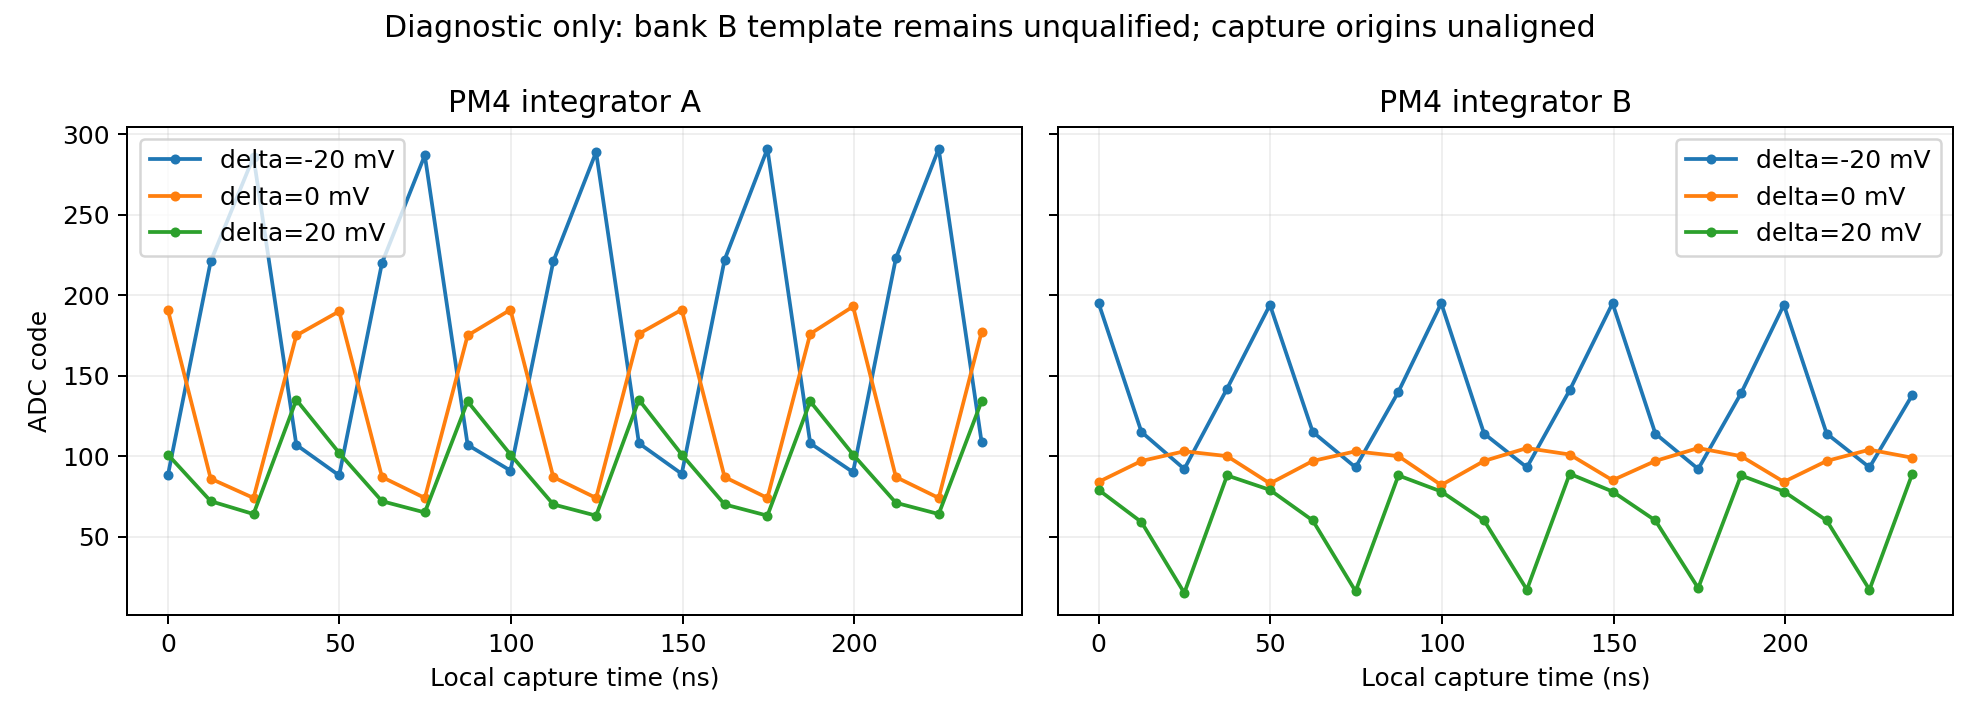
\includegraphics[width=\linewidth]{group14-integrator4-diagnostic.png}\end{center}
